\chapter{Alignments with Pair HMMs}\label{CHAPTER:PAIRHMM}

In this chapter we will describe scoring schemes for pair alignment using pHMMs
or GpHMM. Scoring schemes will differ in two conceptual ways. One way is in the
used model and the second is in the decoding algorithm. At first we show how the
pHMMs can be used to sequence alignment, after that we describe decoding methods
that can be used to reconstruct alignment. The last part of this chapter will
discuss several uses of pHMM and GpHMM to sequence alignment or to the related
problems.

\section{Usage of Pair Hidden Markov Models}\label{SECTION:SIMPLEPHMM}

We can divide states of pHMM into three types.  Ones that generates symbol in
both sequences (match states), states that generates symbol in only one sequence
(indel states) and silent
states. If pHMM generates  symbols in both sequences we consider those symbols
to be homologous. We will consider symbols that were not generated by such state
as indels. Alternative view is to imagine that indel states generate symbol in
one sequence and gap symbol in the second sequence. In such view pHMM generates
an alignment.

Now we show classical pHMM for sequence alignment. It is equivalent to scoring
scheme of Needleman-Wunch algorithm with affine gap model. It consists of three
states: one that generates aligned pairs, and two states for generating
indels (one for each sequence). Model is shown in figure \ref{FIGURE:SIMPLEPHMM}. 

\begin{figure}
\begin{center}
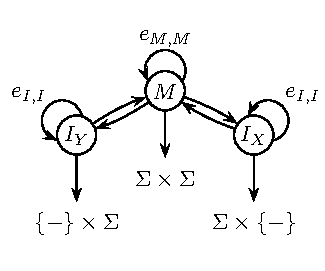
\includegraphics{../figures/pairHMM.pdf}
\end{center}
\caption[Simple pair HMM model for alignment]{Pair hidden Markov model for pair alignment. It has two transitions
parameters $e_{M,M}$ and $e_{I,I}$, since we set $e_{I,M} = 1 - e_{I,I}$ and
$e_{M,I}=\frac12-\frac12e_{M,M}$. Match state $M$ generates aligned pair of symbols
and states $I_X$ and $I_Y$ generates symbols only in $X$ or $Y$ respectively.
Initial distribution is even.
}\label{FIGURE:SIMPLEPHMM}
\end{figure}

As mentioned before, score of the alignment is the probability of state path
that correspond to such alignment. Therefore we can find the alignment with
highest score by two dimensional version of Viterbi algorithm. Advantage of
using this model instead of the Needleman-Wunch algorithm is that pHMM gives
probabilistic explanation of the alignments. 

In following sections we will review several pHMMs and GpHMMs that were used to
sequence alignments or other purpose, for example gene finding. We will review
the application domain of the model, its topology, decoding function, parameter
estimation and optimisation heuristics. But at first, we have to introduce small
biological background.

\todo{zadefinuj quality of an alignment}

\section{Decoding Methods}

In this section we review three decoding methods that were successfully used to
get reconstruct pairwise alignment: the Viterbi algorithm, the Posterior
decoding and the Marginalized posterior decoding.

Let $H$ be an pHMM (or GpHMM) and $X$ and $Y$ be the sequences that we want to
align. The probability $\prob{X,Y\mid H}$ is the probability that $X$ and $Y$
are aligned under model $H$.  From path $\pi$ (or state path and the
sequence of durations in case of GpHMM) we can reconstruct unique alignment.
Such alignment we will denote by $A_{\pi}$.
  \[\prob{\pi\mid
X,Y,H}=\frac{\prob{\pi,X,Y\mid H}}{\prob{X,Y\mid H}}\] is the probability, that
$A_{\pi}$ is alignment of $X$ and $Y$ under the condition, that $X$ and $Y$ were
generated by model $H$.  We can use $\prob{\pi\mid X,Y,H}$ as a score of an
alignment $A_{\pi}$. Such $\pi$ can be found by the two-dimensional Viterbi
algorithm. $A_{\pi}$ can be constructed from $X,Y$ and $\pi$ in straightforward
way: for every match state from $\pi$ (that generated $X[i]$ and $Y[j]$) we add
column $(X[i],Y[j])$. For every indel state in $\pi$ that generates $X[i]$ we
add to alignment column $(X[i],'-')$. Indel state for the second sequences are
analogous.  The two-dimensional Viterbi algorithm is used in the most of the
applications we will discuss later.

Now we show two variants of the Posterior decoding for the pHMMs (the Posterior
decoding and the Marginal posterior decoding).  Let $\prob{X[i]\sim Y[j]\mid
X,Y,H}$ be the probability that $X[i]$ and $Y[i]$ are aligned (sum of the
probabilities of all alignments which contains column $(X[i],Y[i])$. Let
$\prob{X[i]\sim -_j\mid X,Y,H}$ be the probability that $X[i]$ is aligned to a
gap that is in $Y$ between positions $j$ and $j+1$ and let $\prob{-_i\sim
Y[j]\mid X,Y,H}$ be the probability that $Y[j]$ aligned to gap in $X$ between
positions $i$ and $i+1$.  Similarly, let $\prob{X[i]\sim - \mid X,Y,H}$ be the
probability that $X[i]$ is aligned to a gap at any position and let $\prob{-\sim
Y[j]\mid X,Y,H}$ be the probability that $Y[j]$ is aligned to a gap at any
position.  Posterior probabilities defined above can be computed by the
two-dimensional version of the Forward-Backward algorithm (probability that
symbol is aligned to any position is the sum of the probabilities that symbol is
aligned to a gap at position $i$ for all possible positions $i$).

Let alignment $A$ of an sequences $X$ and $Y$ has length $n$ and
consists from columns $a_0,a_1,\dots a_{n-1}$. Each column $a_i$ is pair
$a_i=(x_i,y_i)$ where $x$ and $y$ is either symbol from $\Sigma$ or a gap
symbol\footnote{Note that $x$ and $y$ can't be both gap symbols.}.
Let $d_A^x(i)$ be the number of non-gap symbols in $x_0,x_1,\dots x_i$
and $d_A^y(i)$ be the number of non-gap symbols in $y_0,y_1,\dots, y_i$ and
$d_A^x(-1)=d_A^y(-1)=0$. Intuitively, $A[0:i]$ is alignment of $X[:d_A^x(i)]$ 
and $Y[:d_A^y(i)]$. Then the posterior probability of an alignment column is
\[P(a_i)=
\begin{cases}
\prob{X[d_A^x(i)-1]\sim Y[d_A^y(i)-1]\mid X,Y,H} & \text{if $x_i$ and $y_i$ are not gap symbols}\\
\prob{X[d_A^y(i)-1]\sim -_{d_A^y(i)-1}\mid X,Y,H}  & \text{if $y_i$ is gap symbol and $x_i$ not}\\
\prob{-_{d_A^y(i)-1}\sim Y[d_A^y(i)-1]\mid X,Y,H}  & \text{if $x_i$ is gap symbol and $y_i$ not}
\end{cases}
\]

The \abbreviation{Posterior decoding}{PD} find the alignment $A=a_0a_1\dots
a_{n-1}$ that maximizes
the product of the posterior probabilities of it's columns: 
\[A = \arg\max_{A'\in Al(X,Y)}\prod_{0\leq i <
|A'|}P(a'_i)\] where $Al(X,Y)$ denote the set of all  alignments of a sequences
$X$ and $Y$. Similarly we can define \abbreviation{Marginalized posterior
decoding}{MPD}: Let $P'(a_i)$ is the marginalized posterior probability:
\[
P'(a_i) = \begin{cases}
P(a_i) & \text{if $x_i$ and $y_i$ are not gap symbols}\\
\sum_{0\leq j < |Y|}\prob{X[d_A^y(i)-1]\sim -_{j}\mid X,Y,H}  & \text{if $y_i$ is gap symbol and $x_i$ not}\\
\sum_{0\leq j < |X|} \prob{-_{j}\sim Y[d_A^y(i)-1]\mid X,Y,H}  & \text{if $x_i$ is gap symbol and $y_i$ not}
\end{cases}
\]
Then the MPD find alignment $A=a_0a_1\dots a_{n-1}$ that maximizes
\[A = \arg\max_{A\in Al(X,Y)}\prod_{0\leq i < |A'|)}P'(a'_i)\] 
where $A'=a_0a_1\dots a_{k}$ for some $k$.

The Posterior decoding and the Marginalized posterior decoding were used by
Lunter {\it et al.} and both produced better alignments then alignments founded
by the Viterbi algorithm (the measure in which those alignments were better will
be described later). Once posterior probabilities of all possible columns of an
alignments are computed, we can found the alignment that maximized the desired
function in $O(|X||Y|)$ time \cite{Lunter2008}. 

%Other decoding method can be done by the poster
%Other option is to
%use the  Posterior decoding: for every pairs of residues $X[i],Y[j]$ we compute
%posterior probability that $X[i]$ and $Y[j]$ are aligned $\prob{X[i]\sim Y[j]\mid X,Y,H}$.
%Score of an alignment is sum of posterior probabilities of the aligned residues.
%Later in this chapter we show different variants of the Posterior decoding for
%pHMM.


\section{Pair Hidden Markov Models And Gene Model}

In this section we describe several pair hidden Markov models (or generalized
pair hidden Markov models) with gene structures incorporated into their
topology. These models were used either to alignment of coding DNA or proteins
to genome or to the comparative gene finding.

TODO: Tu bude mega obrazok (asi na jednu stranu), kde budu nakreslene rozne
topologie.

%\subsection{Genes}

%Gene, codon, exon, intron, triplets,..., evolution rate, splice site

At first we introduce several comparative gene finders. Comparative gene finders
use evidence from two organism to find genes. They use pHMM to simultaneously  
align and annotate sequences. 

\subsection{DoubleScan}
Meyer {\it et al. (2002)} developed comparative gene DoubleScan.
Generally, DoubleScan has three types of
states: {\it match} states, which generated same number of symbols in both
sequences;   {\it emit} states, which generate sequences only in one sequence
and silent states. DoubleScan's HMM contains structures for exons, introns and
intron-like structures that are outside genes. 

Basic structure of GpHMM consists from three types of substructures:
substructures that emits exons, substructure that emits introns and substructure
that generates intergenic regions. Each structure was in the alignment three
times: once from match states and twice as emit states. Exon substructure was
single state emitting codons (triplets that will be translated into proteins).
There was one additional intron substructure that was connected to states that
generated intergenic regions. This additional intron substructure was in the
model to avoid detecting of pseudogenes. This GpHMM has $54$ states.

%Every such
%structure has three version: one matching version, which emit aligned residues
%and one structure per sequence to emit indels.  Overview of DoubleScan's HMM
%structure is in figure \ref{}. 
\nocite{Meyer2002}

Emission probabilities if the {\it match exon} state were estimated from
relative frequencies in the training set with Dirichlet priors
\cite{Meyer2002,Durbin1998}.  Emission probabilities of other states were
generated  by marginalizing emissions of the match exon state. Transition
probabilities from initial state were even, transition probabilities for splice
sites were estimated by splice site predictor. Other transitions were observed
from train data and tuned by hand.

DoubleScan uses Viterbi algorithm as decoding method.  To reduce running time of
Viterbi algorithm they use stepping stone algorithm: at first they run BLASTN to
find local alignments. Then DoubleScan choose consistent subset of matching by
greedy method described in section \ref{SECTION:SSA}. They restrict Viterbi
algorithm to such subset allowing tolerance 15 bases.

\subsection{SLAM} 

\begin{figure}
\begin{center}
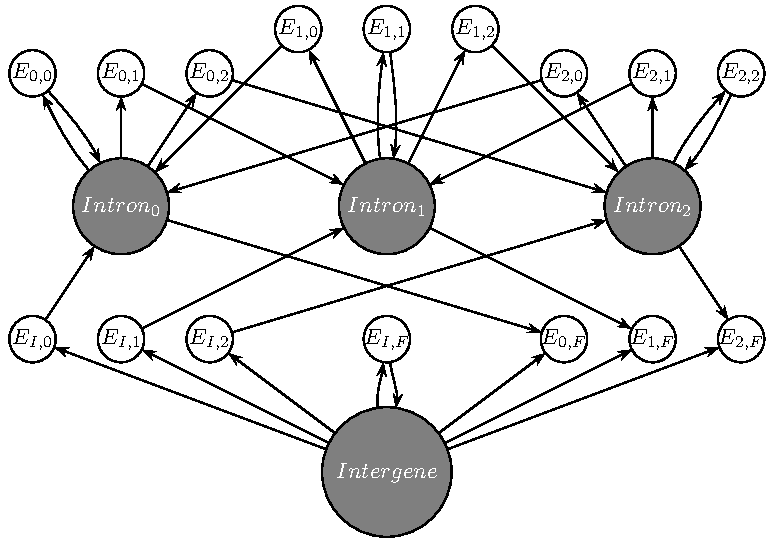
\includegraphics{../figures/slam.pdf}
\end{center}
\caption[HMM topology of SLAM's GpHMM]{
Topology of GpHMM used by SLAM (states for genes on reverse strand are omitted).
Gray states has geometric distribution (modeled with self-loop which are omitted
in the figure). Emissions of shaded states are done with three state pHMM. White
states econdes exons. Each has associated duration distribution and emmisions
are done also with three-state pHMM ($5$-th order that emitted codons at once).
Since introns can be inside codon model contain exon state for every possible
interruption: $E_{i,j},0\leq i,j<3$ is exon that begin with end of the prevous
exon of length $((3-i)\mod 3)$ and end with the beginning of the exon with
length $j$. $I$ stands for start codon and $F$ stand for stop codon: states
$E_{I,\cdot},E_{\cdot,F}$ and $E_{I,F}$ models exons adjecent to the begininning
and the end of a gene.  $Intron_i$ models intron that interrupted codon on
$i$-th position ($0$ means that intron is not interrupting any codon).
}\label{FIGURE:SLAM} \end{figure}

SLAM \cite{SLAM2003}  is comparative gene finder based on generalized pair
hidden Markov model \cite{Alexanderson2004} with some states being also a
high-order states (with dependence on previous emissions).  It predicts gene
structures for pair of related eukaryotic organisms. SLAM's decoding method is
Viterbi algorithm. 

Unlike DoubleScan, SLAM defines true GpHMM because state durations are not
constant, but are sampled from some distribution (however, distribution they
used in not specified). Topology of the model can be found in figure
\ref{FIGURE:SLAM}.
Emission of pairs of codons were assigned from codon-based PAM matrix.


To reduce running time of the algorithm, they restrict the computation of
alignment in following way: At first they  align input sequences using AVID
alignment tool\cite{Bray2003} to get anchor alignment. They restrict the Viterbi
algorithm in such way, that it could align  in a way, that every base from
bases were extended to intervals of size $3$ bases of bases surrounding each
matching base.



\subsection{Twain}

TWAIN is another approach to use GpHMM to find genes \cite{Majoros2005} and is
interesting because of it's decoding algorithm. Twain GpHMM have two type of
states: the states with fixed durations (which emit sequences of fixed length)
and the states with the variable duration lengths which are associated with some
distribution.  The states with fixed durations corresponds to the specific
signals line splice sites, start/stop codons, donor sites and so on.
Additionally, the states with variable duration are not connected with each
other; the transitions from/to such states are only to/from states with fixed
duration lengths. Therefore if we know the positions of all signals in the
sequence, we know that sequences between signals were generated by one state.
This can be exploited in following way.

TWAIN at first annotate input sequences using gene-finder TIGRscan
\cite{Majoros2004} (each sequences is annotated independently) which finds
signals in the sequences and create parse graph: vertices of the parse graph are
the signals in the sequence (each signal correspond to a state of GpHMM).  Two
signals are connected with edge if in the genome one signal can follow another:
for example start codon can be followed by the stop codon or donor site.
Therefore start codons are connected with edge with following stop codons and
donor sites. Each edge is scored by the probability of the most probable state
path between those two states in the TIGRscan's HMM. To reduce the size of the
graph, some edges are omitted by heuristic.

TWAIN created graph $G$ by cartesian product of two parse graphs and omit the
vertices that corresponds to pairs of different signals since they are unlikely
to be seen in the alignments. Each node in the graph correspond to the state $s$
of the GpHMM and cell $c$ in the dynamic programming matrix of the Viterbi
algorithm. TWAIN assumes that sequences corresponding to cell $c$ were generated
by the state $s$.  Edges between cells $c_1,c_2$ correspond to alignments
generated by single state from GpHMM (since states for $c_1$ and $c_2$ are
connected through generalized states).  The Viterbi algorithm is computed only
on cells corresponding to graph $G$ which significantly reduce the computational
complexity \cite{Majoros2005}.

%At first twain annotated input
%sequence with the gene-finder TIGRscan to construct parse graph. Vertices of the
%parse graph are specific signals (splice sites, start codon, stop codon,
%promoters, \dots) with their positions in the genome.  Edges in the parse graph
%are between signals that can be adjacent in the gene.  For example there are
%edges from the start codons to the following stop codons, 3' splice sites, and
%so on. Not all such edges are permitted in the parse graph, for example for
%non-coding predecessors edges only the top $r$ scoring edges are preserved.
%
%When the parse graph of both sequences is computed
%
%It uses interesting technique to improve
%running time of the algorithm. It search in the both sequences for the signals
%(like ...,..,..,). After that it creates graph: two signals in one sequence are
%connected by an oriented edge if one signal can follow other signal. They do
%Cartesian product of such graph of both sequences. Resulting graph is used to
%restrict search space of the sequence alignment.
%TODO

\subsection{GeneWise}

GeneWise predict genes by aligning protein (\correction{or profile HMM}{nikde to
nie je spomenute, ze co to je}) to similar gene structures in DNA
\cite{GeneWise2004}. Instead of pHMM defined as in section \ref{SECTION:PAIRHMM}
it used probabilistic transducers. Probabilistic transducer are very similar to
pHMM. They are both probabilistic finite state machines but unlike pHMM which
are generating two sequences, probabilistic transducers transform one sequence
into other sequence.  Second difference is that transducers have ``emissions''
associated with transitions, not with states.  Therefore the ``emission'' of
transducer $e_{u\to v,(x,y)}=p$ means that during transition $u\to v$ symbol $x$
is read from the input sequence ($x$ has to be on the input) and symbol $y$ is
written to the output probability $p$ ($x$ and $y$ might be also gap symbol and
in such case it represents insertion or deletion).  While pHMM defines
distribution $\prob{X,Y\mid H}$, the probabilistic transducers defines
distribution $\prob{X\mid Y,H}$, the probability that sequence $Y$ will be
transformed into sequence $X$.

Advantage of transducers over the pHMM is that they easily allow compositions of
such models together with probabilistic interpretation of the compositions.
Composition of two transducers $A$ and $B$ is transducer $C$ that transform
sequence $X$ into sequence $Y$ using transducer $A$ and then it transform $Y$
into sequence $Z$ using transducer $B$. %The probability that $X$ is transformed
%into $Z$ using $C$ is $\sum_{Y}\prob{Y\mid X,A}\prob{Z\mid Y,A}$.

%Main difference in their model was that emissions were defined for transitions
%and not for states.  
Model was created by composition of the gene prediction model $S$ which
translates genomic sequence into protein sequence and protein homology model $T$
which maps protein sequence into homologous protein sequence.
%While model $S$ translates DNA into protein sequence, $T$ was simple pHMM

Gene prediction model $S$ consists from the single exon state which translates
series of codons into amino-acids. Advantage of It has three submodels for
modeling introns, each from $3$ states. In introns they model splice sites, 
poly-pyrimidine tract and central intron section.
%Each consists from $5$ sections : 5J splice site, central intron section,
%poly-pyrimidine tract, a spacer following the poly-pyrimidine tract and the 3J
%splice site. These $5$ sections are modeled by $4$ states and transitions
%between them

Protein homology model $T$ was simple pHMM from section \ref{SECTION:SIMPLEPHMM}
defined over protein alphabet.  The composition of the models $T$ and $S$ has
$30$ states. Authors removed unnecessary states and they also removed
poly-pyrimidine states to reduce the number of states and transitions
\cite{GeneWise2004}.

%Combined model was created by composition of models $T$ and $S$, from which were
%removed unnecessary states. To decrease state space even more, they remove more
%states, for example poly-pyrimidine states. More details are in
%\cite{GeneWise2004}.

%Parameters for match and insert transitions were derived from amino acid
%distribution from the model $T$, from the codon bias in the organism and there
%was allowed one substitution error while translating codons to amino acids (due
%sequencing errors).


\subsection{Pairagon}

\begin{figure}
\begin{center}
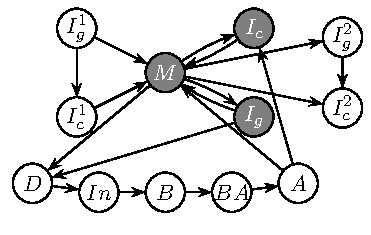
\includegraphics{../figures/pairagon.pdf}
\end{center}
\caption[Topology of Pairagon generalized pair hidden Markov model.]{
Topology of Pairagon GpHMM. All states with excetion to states
$D,B$ and $A$ have self transition.
Shaded states corresponds to the exons: $M$ emits
aligned pairs of symbols, $I_c$ is insertion in coding DNA and $I_g$ is
insertion in genome. States $I^1_c,I^1_g,I^2_c$ and $I^2_g$ corresponds to
unaligned parts of the DNA and cDNA in the beginning and the end of the
sequences. States $D,In,B,BA,A$ corresponds to intron structure and stand for 
Donor, Intron, Branch, Branch Acceptor and Acceptor respectively.
Donor site emitted $8$ symbols and acceptor site emitted $6$ symbols.
}\label{FIGURE:PAIRAGON}
\end{figure}


Aim of Pairagon is to do local alignments of \abbreviation{coding DNA}{cDNA} and
genome \cite{Pairagon2009}. By aligning cDNA to genome we are able to study
intron and exon structures.  To do this task, Pairagon's HMM models consists
from simple pair HMM submodel, which aligns cDNA to DNA and $5$ state submodel
for intron structures.  Whole topology is in figure \ref{FIGURE:PAIRAGON}. 

Model was trained using iterative maximum likelihood approach. At first
parameters was trained on the alignments from the \abbreviation{Mammalian Gene
Collection}{MGC}. In this phase the parameters for intron submodel were set by
hand. Then they align more MGC sequences using this model. Final parameters were
estimated from the new alignments.

Decoding was done by Viterbi algorithm. Runtime of the algorithm was improved by
stepping stone algorithm described in section \ref{SECTION:SSA} and memory
requirements were improved using the Treeterbi algorithm \cite{Keibler2007},
which is similar to the On-line Viterbi algorithm discussed in section
\ref{SECTION:ONLINEVITERBI}.


\section{Non-Geometric Indel Models}
\todo{Povedat niekde ze preco je afiinne rozdelenie geometricke}
In simple pHMM described in figure \ref{SECTION:SIMPLEPHMM}, gap's length have
geometric distribution: the probability that gap have length $n$ is
$e_{M,I}e_{I,I}^{n-1}(1-e_{I,I})$ (if we sum out all emissions). The Viterbi
algorithm is usually computed in log-space: instead of computing product of
probabilities of events\footnote{Event is emission or transition.}, we compute
the sum of logarithms of those probabilities, because computation in log-space
is numerically more stable. The Viterbi algorithm for the simple HMM
will became same as the Needleman-Wunsch algorithm.  Gap penalty will be
$\log(e_{M,I})+\log(1-e_{I,I})+(n-1)\log(e_{I,I})$. By setting $d=\log(e_{I,I})$
and $g=\log(e_{M,I})+\log(1-e_{I,I})-d$ we see that this is exactly affine gap
penalty. Therefore we can say that affine gap penalties corresponds to geometric
distribution of indel lengths.

As we mentioned chapter \ref{CHAPTER:ALIGNMENT}, using non-affine gap model can
improve alignment quality.  Problem with geometric distribution (or affine gap
penalties) is that it gave too high penalty for long indels \cite{} Therefore
some other distribution might be more appropriate, for example zeta distribution
\cite{Cartwright2009}, or combination of several geometric distributions to
approximate the distribution of gap length \cite{Gill2004,Gill2006}.

GpHMM are suited for use of arbitrary duration distributions.
On the other hand, GpHMM are slower to decode so we might want to avoid them if
possible.  One way of incorporating different gap distribution into pair hidden
Markov models without using theirs generalized version is to use several (for
example two) indel states for every sequence. For example FASTA
\cite{Bradley2009} and
Lunter {\it et al. (2008)} used two component mixture models: instead of one
indel state for every sequence we use two indel states for every sequence. They
report that this improved quality of alignments.
\nocite{Lunter2008}

Modeling non-geometric distributions with several states can be problematic. Set
of states with same emission distribution used for modeling modeling
non-geometric distribution is called gadget (There are also additional
property: all transitions entering gadget has to either start in same state or
end in same state. Same holds for transitions that leaves gadget. ). Problems
with gadgets and the Viterbi algorithm are discussed in \cite{Vinar2005}. We
describe discuss the example of such problem for the two component mixture
model.

Let $H$ be an simple pair hidden Markov model with two pairs of indel states.
Let $I_1$ and $I_2$ be indel states that generates gaps in the first sequence.
Gaps in alignments (in the first sequence) that are generated by such model has
distribution $d(n)=(a_1p_1^n(1-p_1)+a_2^n(1-p_2)), n>0, d(0)=1-a_1-a_2$ where
$n$ is the length of the gap, $a_1$ and $a_2$ are probabilities of entering
state $I_1$ and $I_2$ respectively and $p_1$ and $p_2$ are probabilities of
remaining in state $I_1$ and $I_2$ respectively. This is equivalent to
generalized pair hidden Markov model $H'$ with one indel state for every
sequence which have $d(n)$ as it's duration distribution. Both models defines
same distributions of alignments (but not distribution of alignments and state
paths) and running the Forward-Backward algorithm or the Forward algorithm will 
give same results. However, alignments constructed by the Viterbi algorithm
can be different for $H$ and $H'$.

Problem is that in the generalized model the Viterbi algorithm gaps of length
$n$ have ``score'' $d(n)$ but in the non-generalized pair hidden Markov model it
will be $m(n)=\max\{a_1p_1^n(1-p_1),a_2p_2^n(1-p_2)\}, n>0$ and
$m(0)=1-a_1-a_2$.  These two scores are different ($d(n)$ is always higher) and
therefore it is possible that the Viterbi algorithm reconstruct different
alignments. Therefore if we are using the Viterbi algorithm, we should either
train such gadget so that $m'(n)$ will be better approximation of $d(n)$ ($d(n)$
is the distribution for the original model) or use generalized pair hidden
Markov model for the Viterbi algorithm.

%co chcem povedat: niekedy je lepsie pouzit iny gapmodel -- jeden pre kratke
%gapy, jeden pre slhe gapy. Preto sa niekedy 

\section{Aligning Sequences with Variable Rate of Evolution}
 
%\subsection{FEAST} 

The rate of the evolution (the expected number of substitution per position in
sequence over some period of time) is not constant for whole genome. It does not
have to be constant even within one gene. FEAST is pairwise local alignment tool
\cite{FEAST2011} that take into account the variable evolution rate. Simple pHMM
from figure \ref{FIGURE:SIMPLEPHMM} is optimized for one fixed rate of
evolution.  FEAST contain $k$ such submodels, each trained for different rate of
evolution.  Submodels are connected with single silent state.  Since FEAST is
local alignment tool, it one additional submodels for generating unaligned pair
of the sequences in the beginning and the end of the sequences.

To construct alignment (either local or global) FEAST uses the Viterbi
algorithm. Like many local aligners, FEAST use seeding heuristics to reduce
computational complexity of finding local alignments.  At first it use six
different space seeds to get candidate seed and extended those seeds using
x-drop heuristic \cite{Altschul1997} using ungapped version of Forward algorithm
during extension (Viterbi algorithm is usually used during extension phase).

Estimation of parameters was done by expectation maximization approach (with
Baum-Welch or Viterbi training). They forced gap parameters to be same in all
submodels.

Using different rate of evolution was also used  in the whole genome aligner
GRAPe \cite{Satija2010}. GRAPe's HMM  consisted from two submodels: one for the
parts of the with fast evolution rate with two component geometric mixture model
for indels and the second submodel for the parts with the lower evolution rate
with the geometric distribution of the lengths of the indels. GRAPe uses the
Posterior decoding as a decoding method.

%Dalsie modely: TWINSCAN, MCALIGN2, WABA, Catwright (zeta function)

\section{Biases In Alignments}

Lunter {\it et al. (2008)} conducted extensive survey concerning biases in
alignment. They considered three types of biases (associated with gaps). These
gap biases are also discussed in \cite{Durbin1998} \todo{Naozaj?}. By
\firstUseOf{true alignment} we mean alignment that corresponds to actual 
evolution history.
\begin{itemize}

\item \firstUseOf{Gap wander} means that gap is in different location that in
true alignment. Is is due to random short similarities around the borders of
a gaps that are indistinquishable from true homologies.
%Lunter {\it et al.} gave
%explicit formula for computing the expected proportion of incorrectly aligned
%regions due to gap wander. \todo{Nie je tento vzorec zbytocny?}
%\[F_w =
%\frac{\sigma}{\gamma}\frac{(4e^{4\sigma/3}-3)(4e^{\sigma/3}-1)}{8e^{4\sigma/3}-3}\]
%where $\gamma$ is the ratio of the substitution rate, $\sigma$, to the indel
%rate, $\sigma$.

\item \firstUseOf{Gap attraction} is caused when two gaps are near each other.
In such case merging those caps and introducing few mismatches might have higher
score. 

\item \firstUseOf{Gap anihilation} occurs when there are two gaps with
same length in both sequences. Since indels are not so common, removing both
gaps while introducing new mismatches might increase score of an alignment.

\end{itemize}

Biases are ordered by their frequency from the most occurring to the least
occurring \cite{Lunter2008}. Now we will discuss their simulation study. We will
not go into all details, we will review only the basic setup of their
experiments and main outcomes of the study.

At first we define one measure of the quality of the alignment:
\firstUseOf{sensitivity} is the ``ratio of the correct alignment columns to all
homologous columns'' \cite{Lunter2008}. 

In the first experiment, Lunter {\it et al.} they
simulate evolution using Jukes-Cantor model with $0.375$ expected substitution
per position (the expected sequence identity is $0.705$) with geometric gap
model. From simulation they obtained sequences with true alignments which they
realigned using the Viterbi algorithm with the same model as was used for the
simulation. Alignment accuracy was lowest for the  columns near gaps ($56$\%)
and the sequence identity for columns near gaps was $85$\% which does not agree
with the expectation  $0.705$\% of the sequence identity. Moving away from gaps
the average sequence identity dropped to the $0.68$\%. The increased sequence
identity near gaps is due to gap wander bias. The gap attraction effect caused
that the number of gaps that are in near each other positions was lower then
expected value (obtained from the used gap model).

They run Viterbi algorithm parametrized by range of the substitution and indel
rates. The maximal sensitivity was obtain for the parameters that were identical
to the parameters of the simulated evolution. However, the sensitivity for the
correct model was only $84$\% indicating that even if we have right evolution
models, some biases in the alignments are inevitable.  

The second experiment study the effect of the use of different decoding methods
and different models on the quality of the alignment (however, we will omit some
models from this review).  The overview of the experiment is following.  Lunter
{\it et al.\nocite{Lunter2008}} simulated evolution with parameters that are
close to parameters of human-mouse evolution. They simulated for example the
large-scale variation of GC content, GC-content dependent indel and substitution
rates and GC-indepependent local substitution rave variation \cite{Lunter2008}.
From simulation they obtained $20,000$ homologous sequence pairs with average
length of $700$ nucleotides. They add the flanking sequences to the generated
sequences of length $100$ nucleotides to simulate local alignments.

\todo{Tento odstavec je skaredo formulovany, treba ho upravit}
After simulation they realigned homologous sequences using the Viterbi algorithm
(VA), the Posterior decoding (PD) and the Marginalized posterior decoding (MPD)
with different models: three state pHMM ($H_S$); $H_S$ with two indel states for
every sequence to get two component geometric mixture gap model ($H_M$) and the
full model with all parameters that were used for simulation ($H_F$) like the
variable indel and substitution rate. 
%After realignment phase they compare new alignments with true alignments
%obtained from simulation.

Now we define two additional measures of the quality of the alignment. The
\firstUseOf{false positive fraction (FPF)} is ``the proportion of the wrongly
aligned columns among all nongapped columns'' \cite{Lunter2008}. ``The
proportion of columns containing padding sequence among all aligned columns'' is
the \firstUseOf{the nonhomologous fraction (NHF)}.


The use of the different models has little impact on the sensitivity of the
constructed alignments. Interesting is that for the full $H_3$ model and the
Viterbi algorithm the sensitivity was lower than with the use of the simple
model $H_1$. With other decoding algorithm the models $H_2$ and $H_3$ has
slightly higher sensitivity then the $H_1$ model. However the FPF  was higher
for the model $H_1$ was lower for $H_2$ and higher for $H_3$.

While the using the ``better'' model does not significantly improve the quality
of an alignments, using the Posterior decoding and Marginalized Posterior
decoding improved the sensitivity by approximately $2.5$\% regardless of the
model. On the other hand the FPF and the NHF was increased with use of the PD
and MPD. The sensitivity of the PD and the MPD were similar but the FPF was
lower for the MPD. 

The main outcome of this experiment that proper decoding method can improve
quality of the alignment while the use of the simpler model doest not
significantly reduce the quality of the alignments. However, Lunter {\it et al.}
in their simulations models only relatively simple model of the evolution. By
incorporating structural information into the alignment models combined with the
use of the right decoding algorithm we can improve alignments.  This will be
discussed in the next chapter. 


